\chapter{Server-Side Implementation}\label{chap:server_side_rewrite}

Chapter~\ref{chap:system_architecture_rewrite} introduced the server as the external perception, memory, and language backend of the system.
This chapter describes its implementation: the FastAPI runtime, API groups, perception pipeline, memory update semantics, provider adapters, translation support, worker control, and dashboard.

\section{Runtime Structure and Application State}\label{sec:server-runtime-structure}

The public server process is a FastAPI application.
It exposes the public API under \texttt{/api/v1}, serves the dashboard under \texttt{/dashboard}, mounts static assets, and opens a WebSocket channel for live dashboard updates.
This HTTP boundary is the only server surface used by Pepper and the dashboard.
The robot client does not construct detector, VLM, LLM, tracking, or memory objects directly.

\begin{figure}[t]
\centering
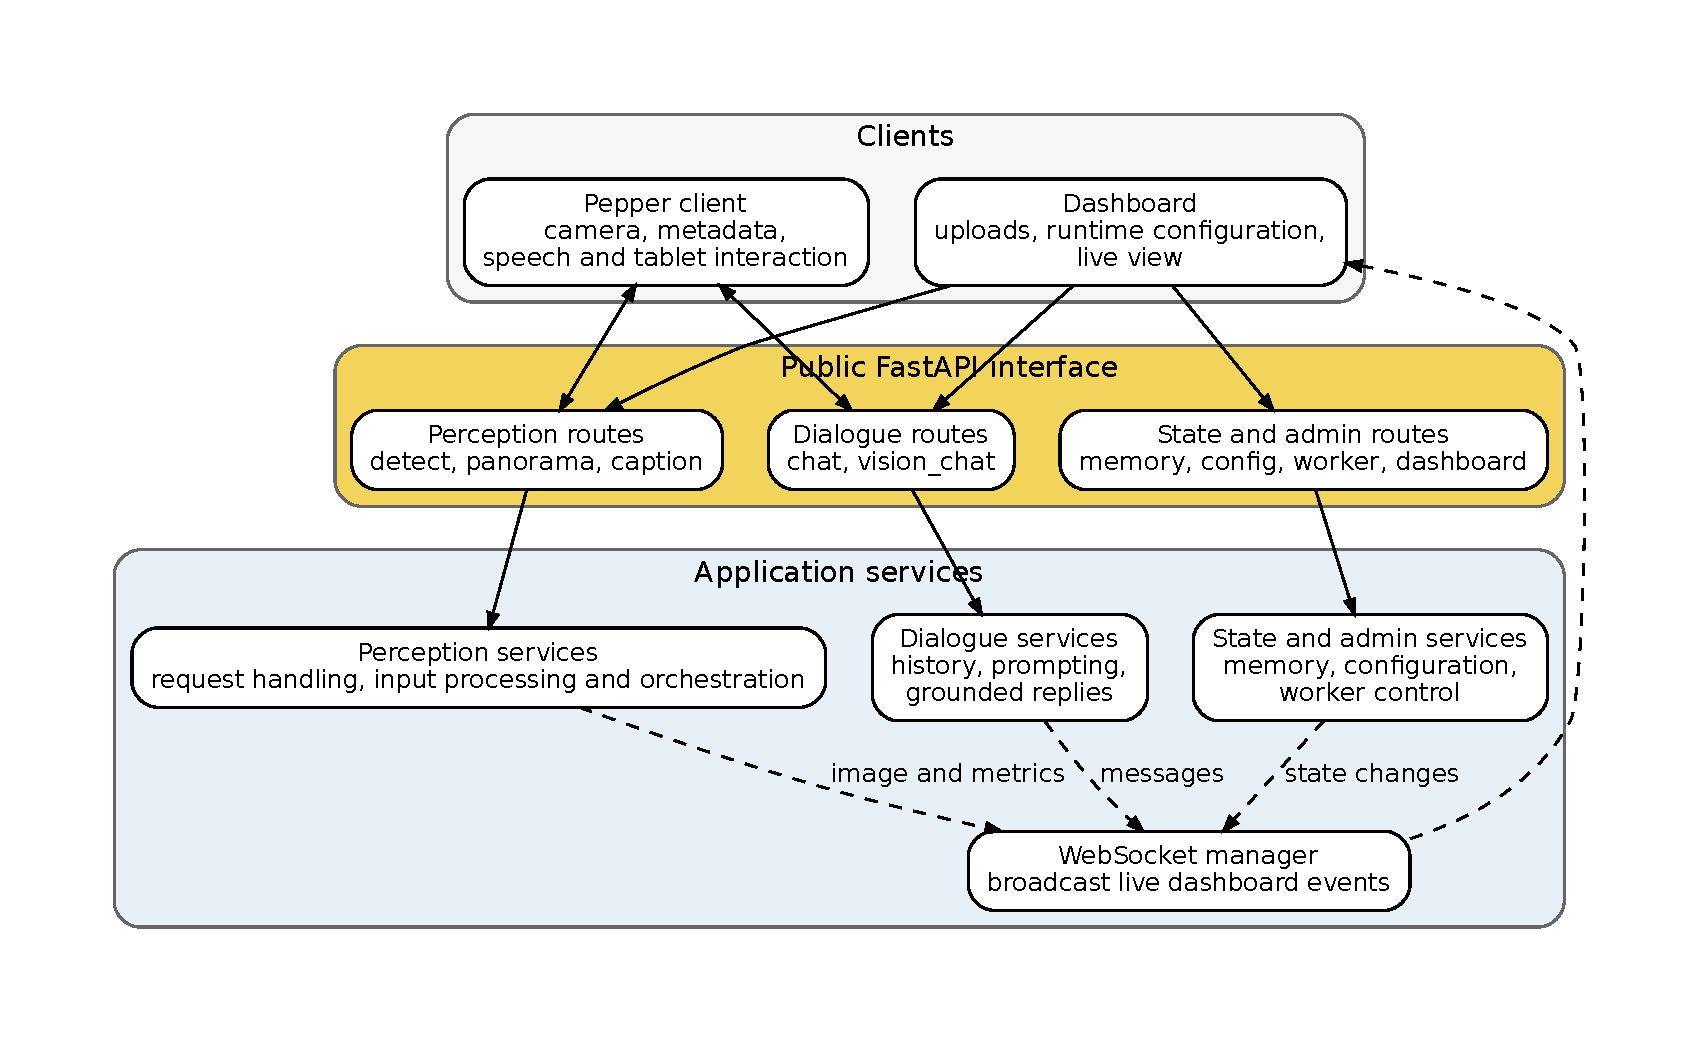
\includegraphics[width=\linewidth]{pics/server_nicer.pdf}
\caption{Server runtime structure. Pepper and the dashboard communicate with the public FastAPI routes. Application services call a runtime adapter, which either uses an in-process perception pipeline or forwards the request to an internal worker process.}
\label{fig:server-runtime-structure}
\end{figure}

Figure~\ref{fig:server-runtime-structure} shows the main server components.
The central dependency root is \texttt{AppState}.
It stores the active configuration and version, runtime adapter, chat service, conversation service, caption service, question-answer pool, and last published dashboard state.
Routes and orchestration services resolve their dependencies through this state object instead of constructing model clients themselves.
Configuration, runtime mode, prompts, providers, and memory access are therefore coordinated in one dependency root.

The server supports two runtime modes.
In-process mode keeps the perception pipeline inside the public FastAPI process and is convenient for debugging.
Worker mode starts a second internal FastAPI application and forwards heavy inference requests to it.
This is the preferred deployment mode: detectors, caption models, embedding models, RelTR, and local VLMs can allocate GPU memory that is difficult to release from a long-lived process.
Keeping those models in a worker leaves the public server as a lighter orchestration layer and allows hard configuration changes to restart only the worker.

The route layer does not need to know which mode is active.
It calls a runtime adapter.
The in-process adapter opens the uploaded image and calls the local pipeline.
The worker adapter serializes the same request and sends it to the internal worker API.
Higher-level services use the same public contracts in both modes, while the deployment choice remains hidden behind the adapter.

\section{Public API and Request Handling}\label{sec:server-public-api}

The public API is organized by robot-facing capabilities rather than by model internals.
Detection routes process visual observations, caption routes provide fast scene descriptions, and chat routes answer text questions from scene memory.
Vision-chat routes send an image and question directly to a VLM.
Memory routes expose the current scene state; configuration and worker routes update runtime settings and control the worker process.

The main detection request is a multipart image upload with optional JSON robot metadata.
The image can be resized before inference to control bandwidth and model cost.
The metadata contains values such as head yaw, head pitch, camera field of view, image size, frame identifier, scan identifier, battery state, and Pepper people-perception outputs.
At the API boundary, the metadata is parsed into Pydantic schemas so later pipeline stages receive normalized values rather than ad hoc dictionaries.

The server also supports panorama-style detection for Pepper scans.
A scan request can contain multiple images and matching metadata payloads.
Depending on configuration, the server can process frames independently or stitch them into a wider panorama before detection.
Independent processing avoids stitching artifacts and preserves per-frame geometry.
Panorama processing gives the detector and VLM a broader visual context in one image.
Both modes are supported because Pepper scans by moving its head through several poses rather than by using a wide-angle static camera.

Caption requests are optimized for the quick-look interaction.
The server receives one image and optional metadata, calls the configured caption service, and returns text together with provider and model metadata.
The same request can also trigger the full detection pipeline in the background.
This lets Pepper speak a quick description first, while the server continues updating detections, scene graph relations, memory, and pregenerated questions for later dialogue turns.

Chat requests are text-first but memory-grounded.
The route receives the user query, language information, conversation identifier, and optionally an object-focus label.
It stores the original user message, builds the model-facing message history, asks the chat service for an answer, stores the assistant response, and broadcasts the message to the dashboard.
Keeping original and model-facing text separate supports bilingual interaction, because the user-facing utterance and the prompt language do not always have to be identical.

\section{Perception Pipeline Implementation}\label{sec:server-perception-pipeline}

Figure~\ref{fig:architecture-perception-pipeline} gives the design view of the perception flow.
A configured \texttt{PerceptionPipeline} implements that flow on the server.
The full pipeline can run captioning, detection, tracking and memory association, Set-of-Mark rendering, scene graph generation, question generation, caption memory update, scene graph memory update, and timing finalization.
Each stage appends its name to the executed-stage list and records timing metrics.
These metrics support dashboard inspection and the latency measurements reported in Chapter~\ref{chap:experiment}.

The pipeline has sequential and partially parallel execution modes.
In sequential mode, captioning runs first, then detection, followed by all post-detection stages.
In parallel mode, captioning and detection start concurrently on copied image objects.
The detector call is synchronous, so it is offloaded through \texttt{asyncio.to\_thread} and protected by a detector lock.
This prevents simultaneous access to one detector instance from multiple requests.
Later stages remain ordered because tracking depends on detections, SoM depends on tracked detections, and scene graph generation depends on detections and optionally the caption.

Detection is implemented behind a detector service abstraction.
The configured registry can load YOLO, RT-DETR, RF-DETR, and OWLv2 backends.
Regardless of backend, the rest of the pipeline receives a normalized detection object containing a class identifier, label, confidence, bounding box, and optional object identifier.
This normalization keeps tracking, memory, SoM rendering, scene graph generation, and dashboard publishing independent of model-specific output formats.

The configured thesis setup uses RF-DETR as the default detector.
Threshold and optional non-maximum suppression controls remain available because detector settings affect dialogue as well as vision: a false positive can become a spoken claim, while an overly strict threshold can hide an object visible to the user.

\section{Tracking and Memory Association}\label{sec:server-tracking-memory}

As discussed in Sections~\ref{sec:object-detection-tracking-reid} and~\ref{sec:architecture-scene-memory}, detection is frame-local while dialogue needs persistent references.
The tracking stage turns detections into scene-memory objects.
For every detection, the server extracts a crop, computes a visual embedding, and matches the current detections to existing tracks.
The association uses the Hungarian algorithm with a weighted cost based mainly on visual similarity and partly on image-space geometry.
Label equality is treated as a hard constraint, so an existing chair track cannot silently become a detected person.

Generic object embeddings use \texttt{nvidia/C-RADIOv4-SO400M} by default~\cite{nvidia_cradiov4_so400m_2026}.
For people, the implementation can use the Hugging Face port \texttt{maennyn/personvit-reid-msmt17-vit-s}~\cite{maennyn_personvit_reid_msmt17_2026}, based on the PersonViT project~\cite{hustvl_personvit_2026}.
This separates general object appearance matching from person-specific Re-ID when that mode is enabled.

Matched detections keep old object IDs.
Unmatched detections create new tracks, and dormant unmatched tracks are aged for later pruning.
The tracked detections then continue through SoM rendering and scene graph generation with stable object identifiers.
The server can then treat repeated observations as evidence about the same physical object instead of creating a new object for every Pepper frame.

The memory update stores two kinds of information.
The low-level track keeps fields needed by tracking, such as the latest embedding, crop, bounding box, confidence, hit count, and last-seen time.
The dialogue-facing object state stores fields needed by downstream components: object identifier, label, status, attributes, bounding box, frame identifier, scan identifier, bearing, robot distance, Pepper person identifier, and timestamps.
The separation matters because tracking needs visual features, while dialogue needs compact symbolic state.

\section{Pepper Metadata Fusion}\label{sec:server-pepper-fusion}

Pepper metadata is fused with server detections after tracking.
The client can send head pose, camera field of view, image size, and people-perception records from NAOqi.
People records can include a Pepper person identifier, yaw, pitch, distance, and social cues such as engagement zone, sitting, waving, gaze, smile, or expression.
These signals are noisy, but they contain embodied information that an ordinary object detector does not provide.

The server projects Pepper-reported people into the image coordinate frame.
A detected person is represented by a bounding box, while a Pepper person is represented by angles and distance relative to the robot.
The fusion code compares these two forms of evidence and can bind a Pepper person identifier to a tracked visual object when the match is plausible.
When the binding succeeds, social and distance metadata are attached to the tracked object state.

The implementation also handles the case where Pepper reports a visible person but the detector misses the person box.
In that case, the server can create a synthetic person detection from the robot-reported direction and distance.
This synthetic detection is less reliable than a real visual box, but it preserves a socially relevant fact: Pepper's native perception reported a person in front of the robot.
For a social robot, losing a person completely is often worse than keeping a lower-confidence person hypothesis.

Robot-derived facts become object attributes in scene memory.
A person can receive attributes that encode sitting, waving, looking at the robot, distance, or engagement zone.
These attributes can later be injected into the scene graph as self-relations and serialized into the chat context.
The server therefore connects ordinary image perception with Pepper-specific social perception.

\section{Set-of-Mark and Scene Graph Generation}\label{sec:server-scene-graph-generation}

\begin{figure}[p]
\centering
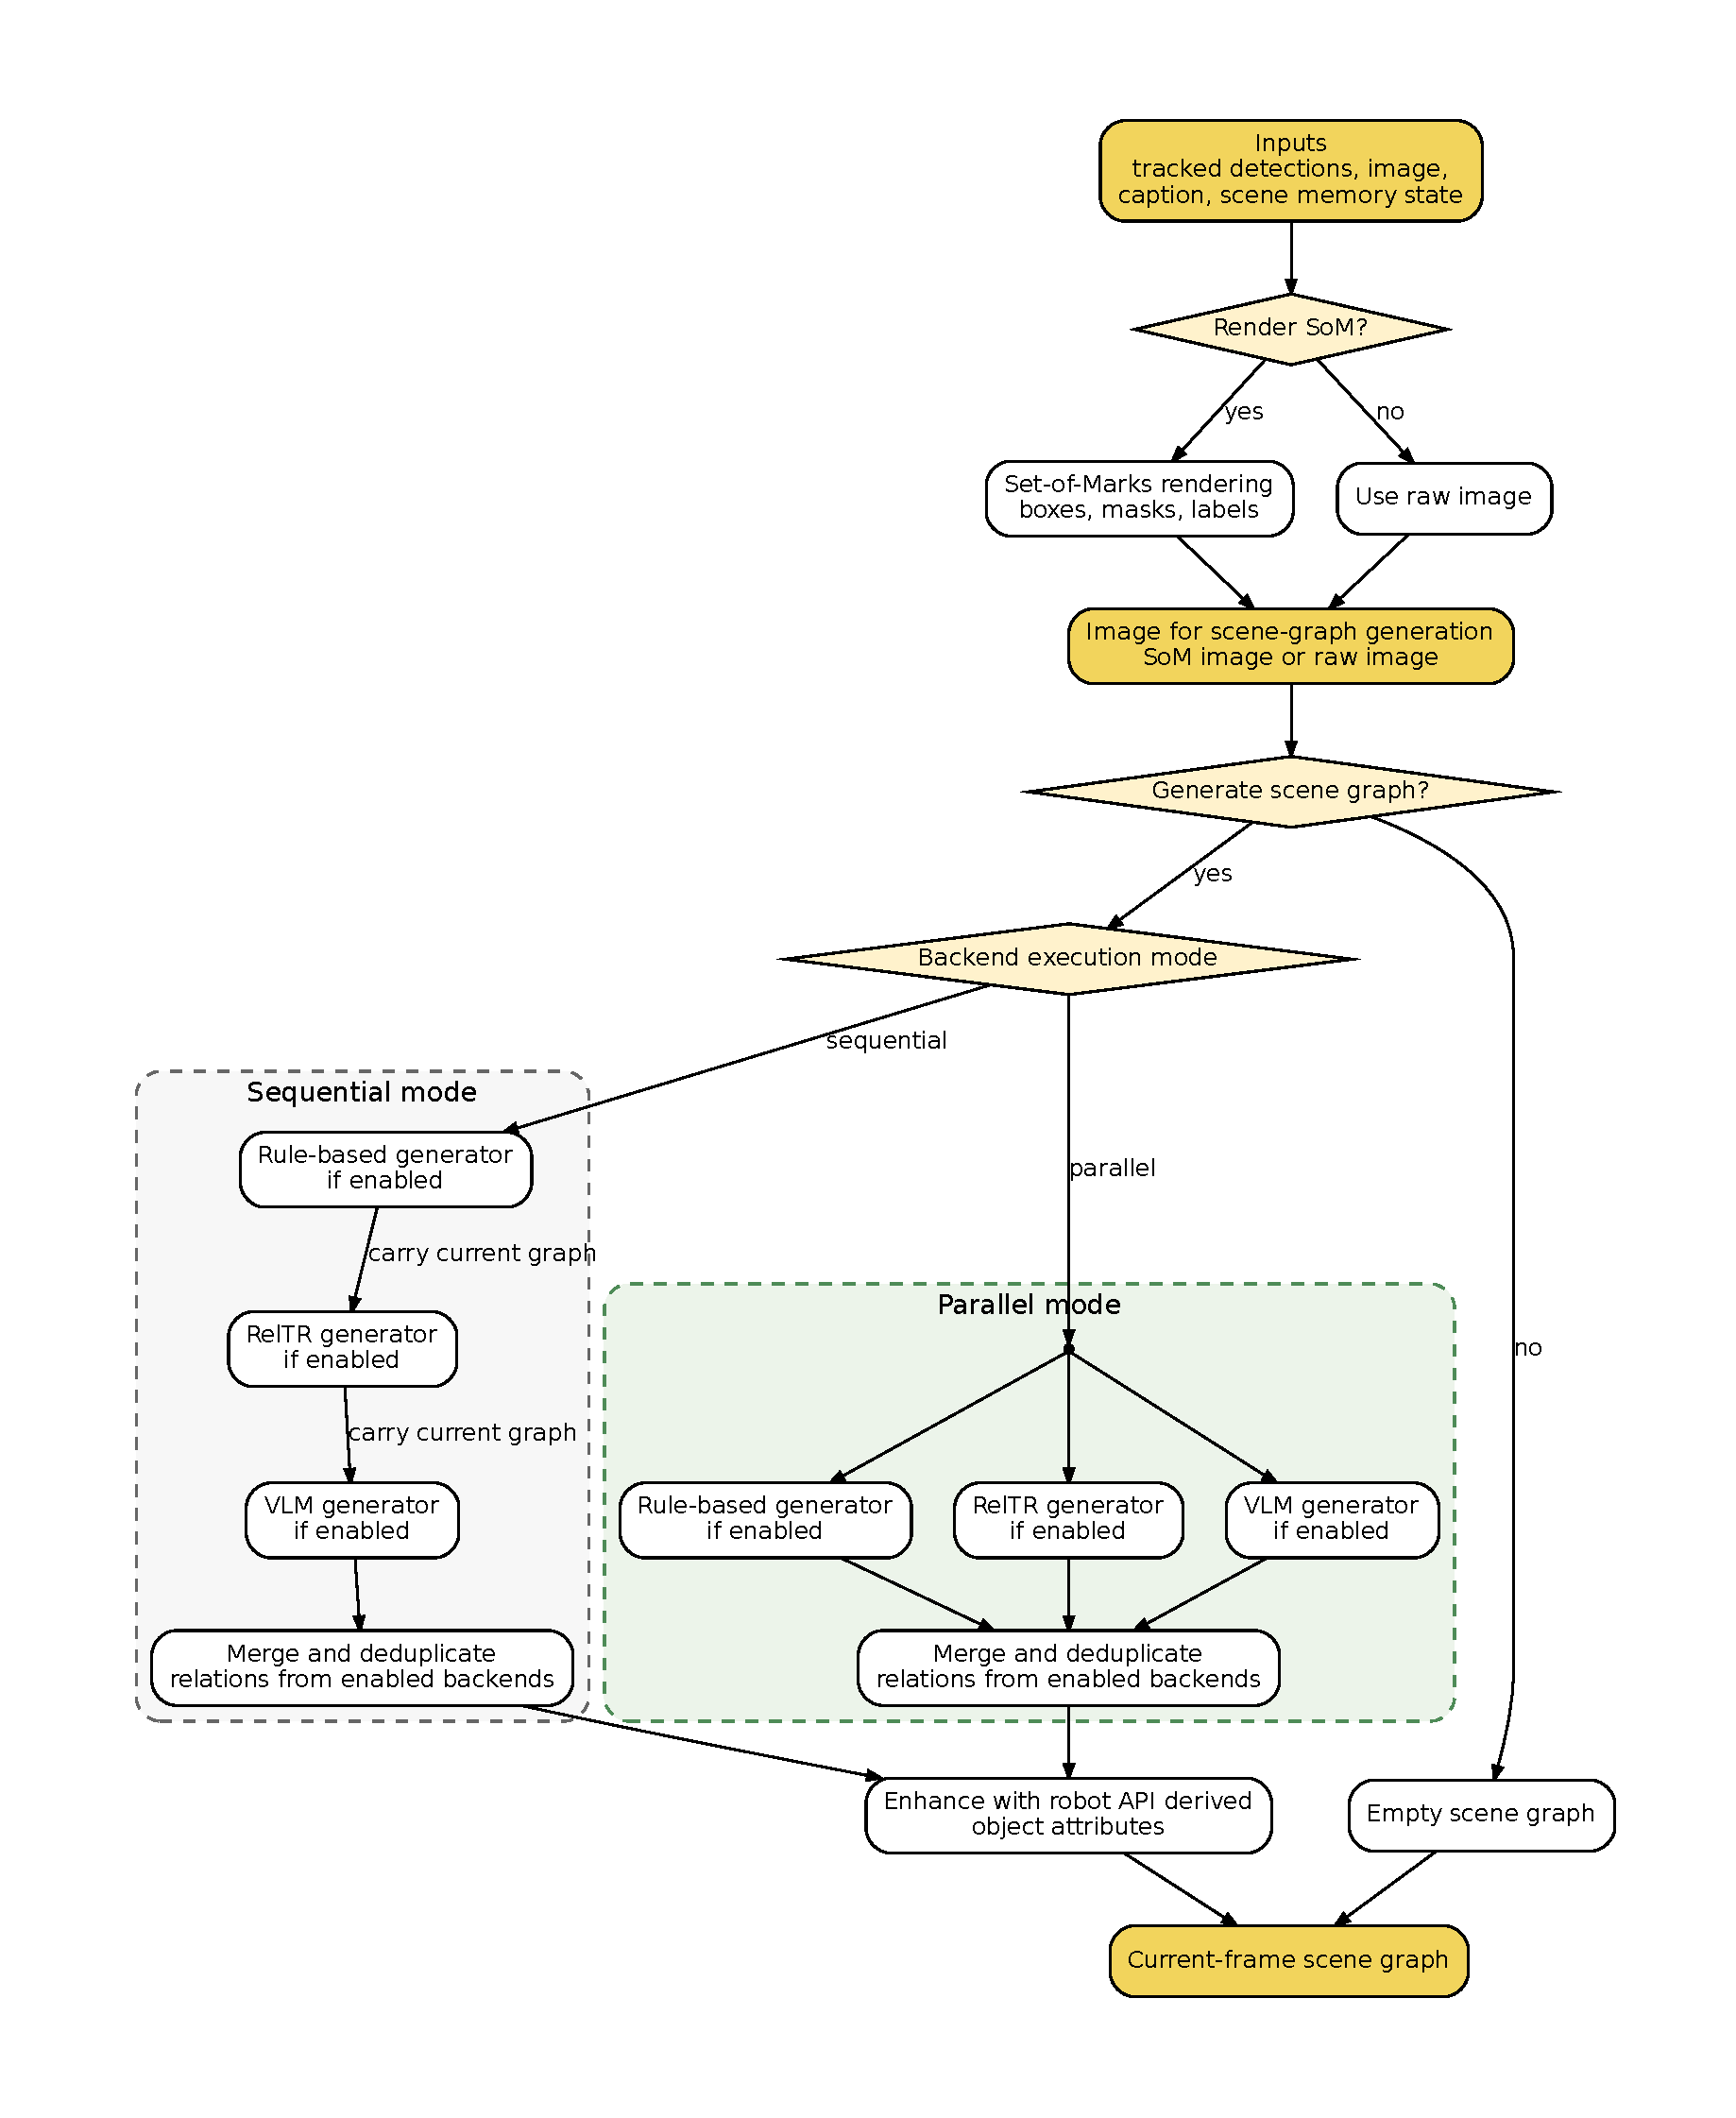
\includegraphics[height=0.78\textheight]{pics/pipeline/04_som_scene_graph_nicer_nicer.pdf}
\caption{Set-of-Mark and scene graph stage. Tracked detections are rendered with persistent identifiers before the VLM scene graph backend is called. Rule-based, RelTR, and VLM relation sources are merged and filtered. Robot metadata can be added to person objects before memory is updated.}
\label{fig:server-som-scene-graph}
\end{figure}

Scene graph generation starts after detections have object identifiers.
The Set-of-Mark painter can overlay boxes, labels, masks, polygons, and object identifiers on the image.
The visual style is controlled by configuration: line thickness, mask opacity, color lookup mode, and mask backend can be changed at runtime.
The mask backend can use lightweight GrabCut or a SAM-based backend with fallback behavior.
The marked image gives the VLM a way to refer to object instances by visible identifiers rather than by ambiguous natural-language descriptions.

The implemented scene graph service combines several optional backends, as shown in Figure~\ref{fig:server-som-scene-graph}.
The rule backend computes deterministic geometric relations from boxes and image crops.
It can produce directional and proximity relations, and it can infer coarse color attributes from object crops.
The RelTR backend proposes learned visual relations and maps predicted subject and object boxes back to the current server detections.
The VLM backend uses the raw or SoM image, prompt templates, the current detections, optional captions, and the allowed vocabulary to generate structured scene graph relations.
Its output is expected as subject--predicate--object triples whose subject and object identifiers refer to tracked detections and whose predicates or unary attributes belong to the configured vocabulary.

Backend execution can be sequential or parallel.
Sequential execution runs rules, RelTR, and VLM in a fixed order.
Parallel execution can offload rules and RelTR to worker threads while the VLM backend runs asynchronously.
The outputs are still merged in deterministic backend order.
The merge is a union with deduplication, followed by enhancement with robot-derived attributes from scene memory.

The VLM backend is deliberately constrained.
It renders prompts from the configured templates, calls the chosen VLM provider, and requests structured output when the provider supports it.
If parsing fails, the backend can ask the model to repair the JSON-like output without resending the image.
After parsing, generated relations are filtered against the current detection identifiers.
Relations that refer to missing or hallucinated object IDs are removed.
Visually plausible VLM output is not automatically grounded in the current tracked object set, so identifier filtering is part of the implementation rather than a cosmetic post-processing step.

Structured output is handled through the same Pydantic schemas regardless of provider.
Cloud LLM and VLM providers use native structured output when available.
Local providers are reached through OpenAI-compatible endpoints.
This covers llama.cpp and Ollama-style servers through the OpenAI API client.
They can use Instructor with \texttt{Mode.JSON}~\cite{instructor_docs_2026}.
In practice, \texttt{Mode.JSON} was more reliable than tool mode for smaller local models, such as GGUF variants of Qwen3.5-0.8B~\cite{unsloth_qwen35_08b_gguf_2026}, which may not implement tool calling consistently.
If provider-native or Instructor parsing fails, the server falls back to requesting JSON text and validating the parsed result against the same schema.

\begin{figure}[!htbp]
\centering
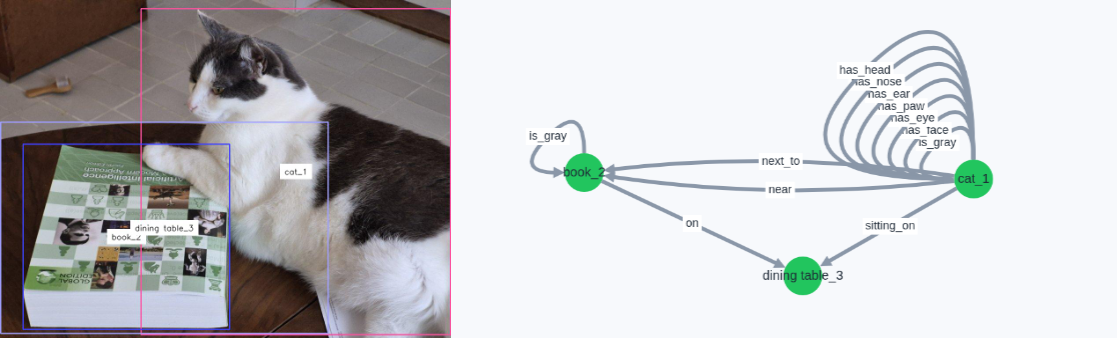
\includegraphics[width=1\linewidth]{pics/sgg_example2.png}
\caption{Example scene graph output. The image is marked with Set-of-Mark identifiers, and the corresponding graph combines detected objects with relations generated by scene graph backends.}
\label{fig:sgg-example}
\end{figure}

Figure~\ref{fig:sgg-example} shows a concrete output of this stage.
The relation is not stored as free text.
It is normalized into graph edges whose subject and object refer to tracked detections.
The result can then be used by memory update, dashboard rendering, evaluation scripts, and later dialogue turns.

\section{Scene Memory and State}\label{sec:server-scene-memory}

Scene memory is the server's in-memory world model.
It stores tracked objects, relationships, captions, object crops, and Pepper person bindings.
The memory lives in the worker process when worker mode is enabled, because that process owns the active perception pipeline.
API services access it through the runtime adapter or a memory proxy, so the public route behavior remains the same in both runtime modes.

Object records contain both visual and embodied fields.
A tracked object can store its identifier, label, status, source, attributes, bounding box, first-seen and last-seen timestamps, hit count, frame identifier, scan identifier, bearing yaw and pitch, Pepper person identifier, robot distance, and engagement zone.
Relation records store a subject identifier, predicate, object identifier, first-seen time, last-seen time, and count.
Caption records store caption text together with provider, model identifier, source, frame or scan identifier, and timestamps.

Scene graph memory update reads numeric graph edges.
If an edge has the same subject and object identifier, it is interpreted as a unary attribute and added to the corresponding object.
If subject and object differ, the edge becomes or refreshes a binary relationship.
Repeated relationships increment their count and update their last-seen timestamp.
Current scene graph backends must therefore preserve correct object identifiers; labels are useful for humans, but numeric IDs make graph memory updates stable.

Memory is bounded by age and capacity.
Objects, relations, captions, tracks, and Pepper bindings are pruned when they become stale or exceed configured limits.
This prevents the robot from treating old observations as current facts.
For example, if a cup was detected several minutes ago and has not been seen again, it should not dominate the next answer as if it were still certainly present.

The memory API exposes this state as a first-class resource.
Clients can request the full scene state, a compact memory summary, object crops, object lists, relation lists, reset operations, and manual create, update, or delete operations for objects and relations.
The memory summary is used by the dashboard and by the robot tablet.
It contains label lists, label counts, graph relations, an SVG graph, and pregenerated question-answer pairs.

\section{Dialogue, Captions, and Question Generation}\label{sec:server-dialogue-services}

The server uses provider adapters for language and vision-language models.
The same orchestration code can use OpenAI, Gemini, local servers with OpenAI-compatible APIs, and local Hugging Face providers where configured.
The abstraction does not erase provider differences, because structured output and multimodal behavior differ between providers.
It gives the rest of the server stable model-client interfaces for chat, VLM, captioning, structured generation, and translation.

The chat service converts scene memory into prompt context.
For general chat, it serializes remembered objects, attributes, relations, and recent captions.
Objects are ordered by a salience heuristic that gives extra weight to people and to social facts such as waving, looking at the robot, engagement zone, distance, recency, and hit count.
The language model is then asked to answer from this context rather than from its parametric knowledge alone.

Object-focused chat builds a narrower context.
If the robot client sends an object label recognized by QiChat, the server matches current memory objects by normalized label and includes the relevant object records and neighboring relations.
If the object has few structured facts but a stored crop is available, the service can request a caption of the crop as a fallback.
This improves object-focused answers when detection succeeded but scene graph generation produced little information about the object.

The conversation service stores recent message history.
It preserves the original user-facing text and the model-facing text separately.
This supports bilingual operation, because a Czech utterance may be displayed and logged as originally spoken while an English or normalized form is used for prompt history.
The same distinction can be kept for assistant responses.

Question generation is a latency optimization.
After scene graph generation, the server can generate a small set of graph-grounded question-answer pairs.
The detection orchestration layer ingests these pairs into a bounded QA pool when memory is updated.
The robot can then expose these questions through the tablet or QiChat dynamic concepts.
If the user asks a cached question, Pepper can answer immediately from the pool; if not, the interaction falls back to ordinary chat.

The vision-chat route is separate from memory-grounded chat.
It sends an image and a question directly to a VLM.
This supports dense visual reasoning that may not be represented in the current graph, but it does not play the same role as the perception pipeline.
It is a direct image-question path, not the main mechanism for maintaining persistent scene memory.

\section{Dashboard, Configuration, and Worker Control}\label{sec:server-dashboard}

% \begin{figure}[p]
% \centering
% 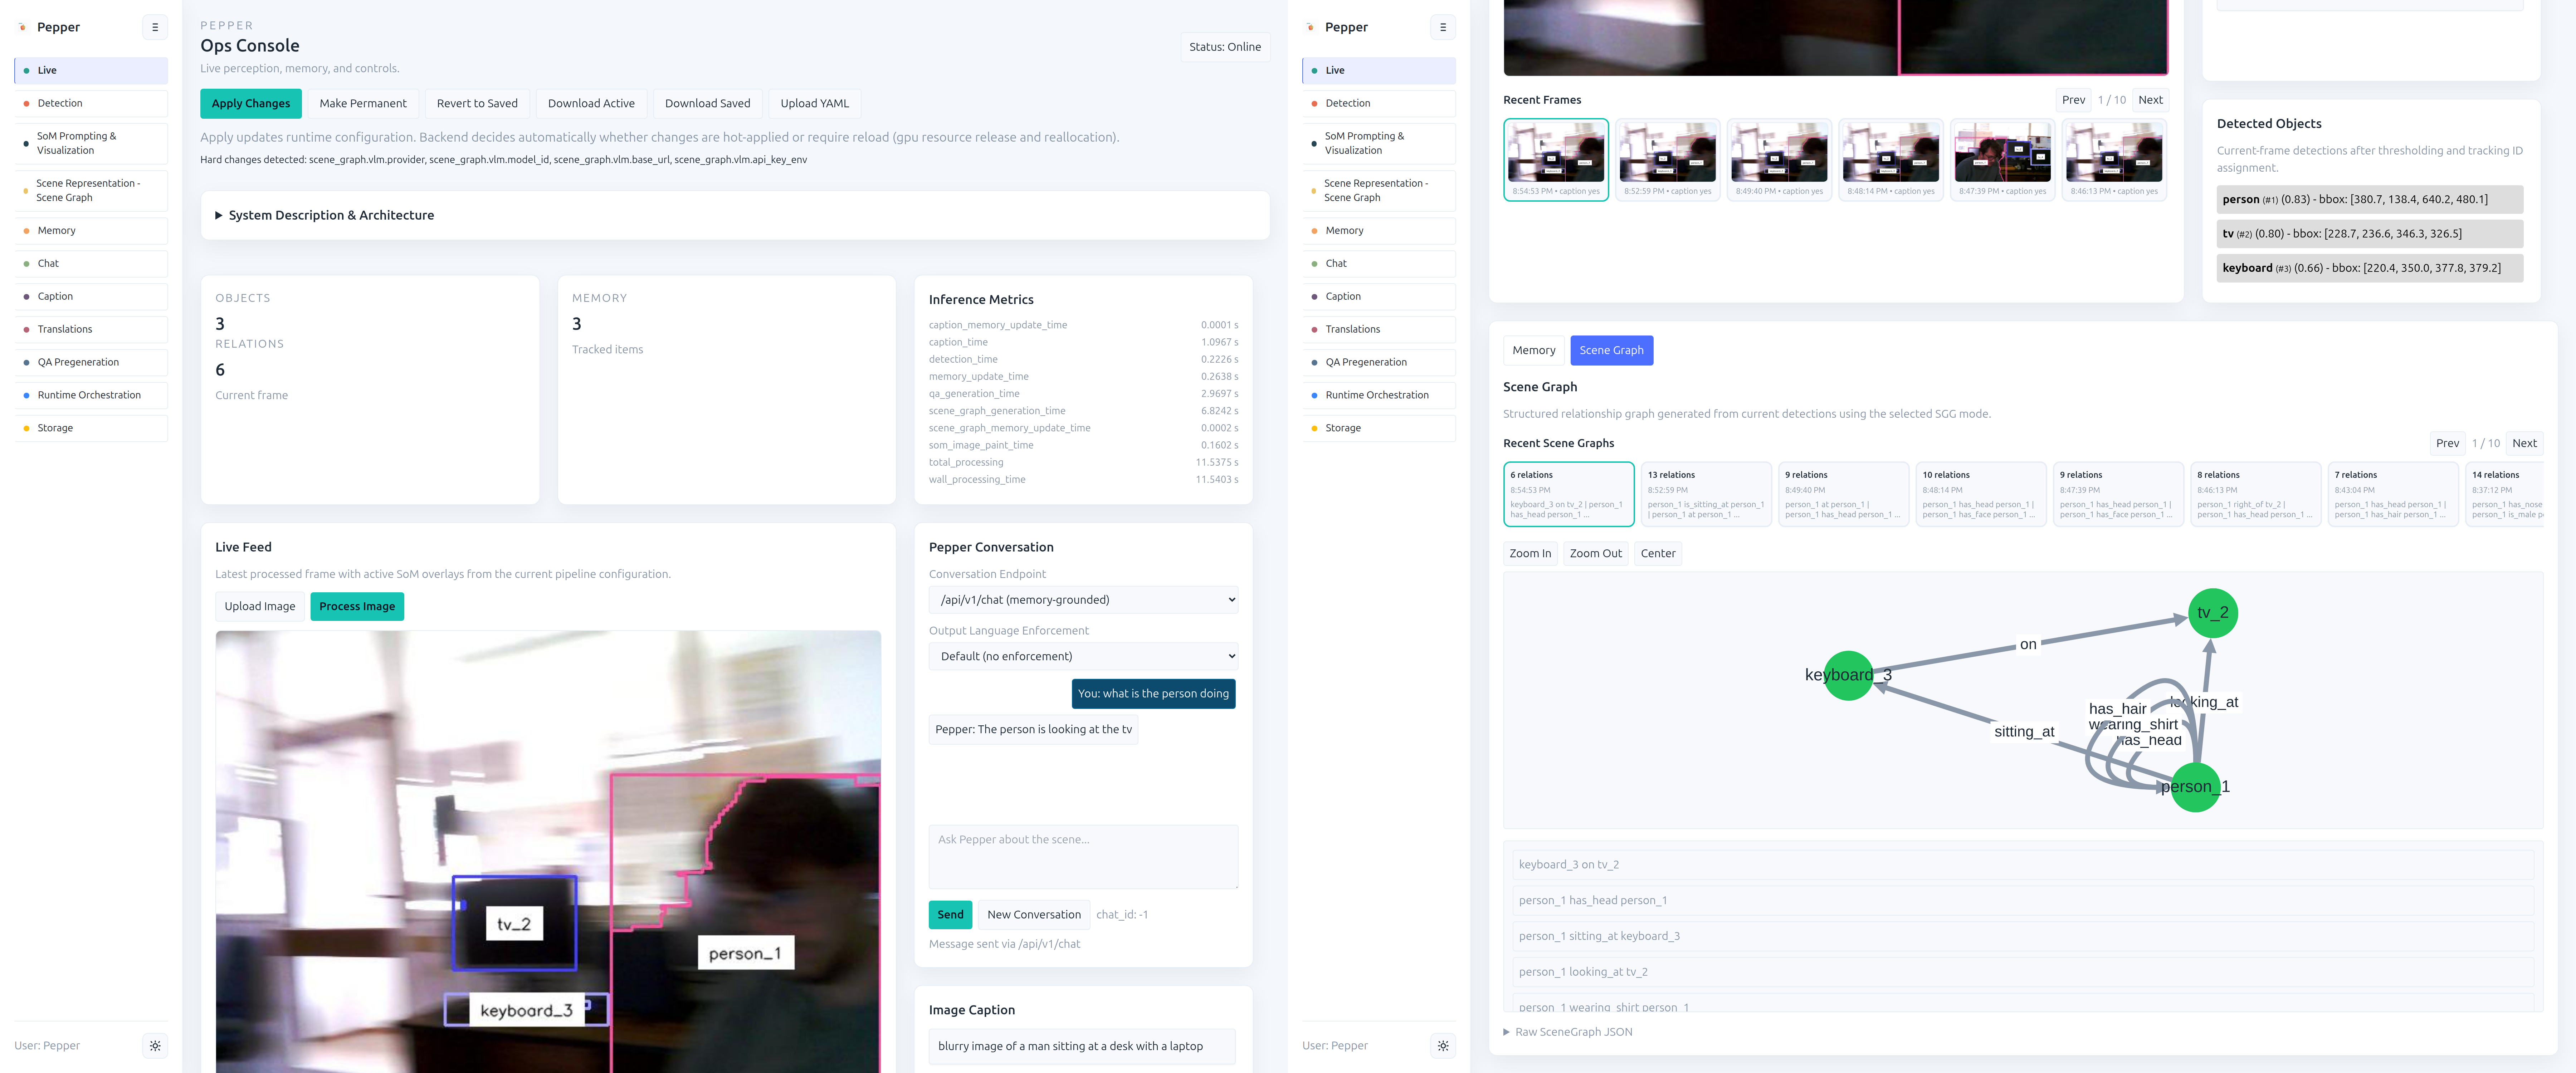
\includegraphics[width=1\linewidth]{pics/dashboard_screenshot.png}
% \caption{Main dashboard view. The dashboard shows the latest robot image, caption, memory graph, object state, chat log, and controls for interacting with the server state during development.}\label{fig:dashboard}
% \end{figure}

The dashboard is the developer-facing view of the same runtime state used by Pepper.
It receives WebSocket events for detections, captions, memory updates, and chat messages.
It also exposes the current image, caption, chat log, memory graph, object lists, relation lists, and generated question-answer pairs.
%Figure~\ref{fig:dashboard} shows the main dashboard page, which is used to inspect the current robot observation and the scene memory built from it.

The dashboard also supports manual interaction with the server.
A developer can send chat messages, inspect model outputs, reset memory, and insert or edit objects and relations.
During testing, a wrong robot answer can originate in several places: robot speech recognition, image capture, detector output, tracking, scene graph generation, prompt construction, translation, or the LLM response.
The dashboard makes those intermediate states visible.

\begin{figure}[p]
\centering
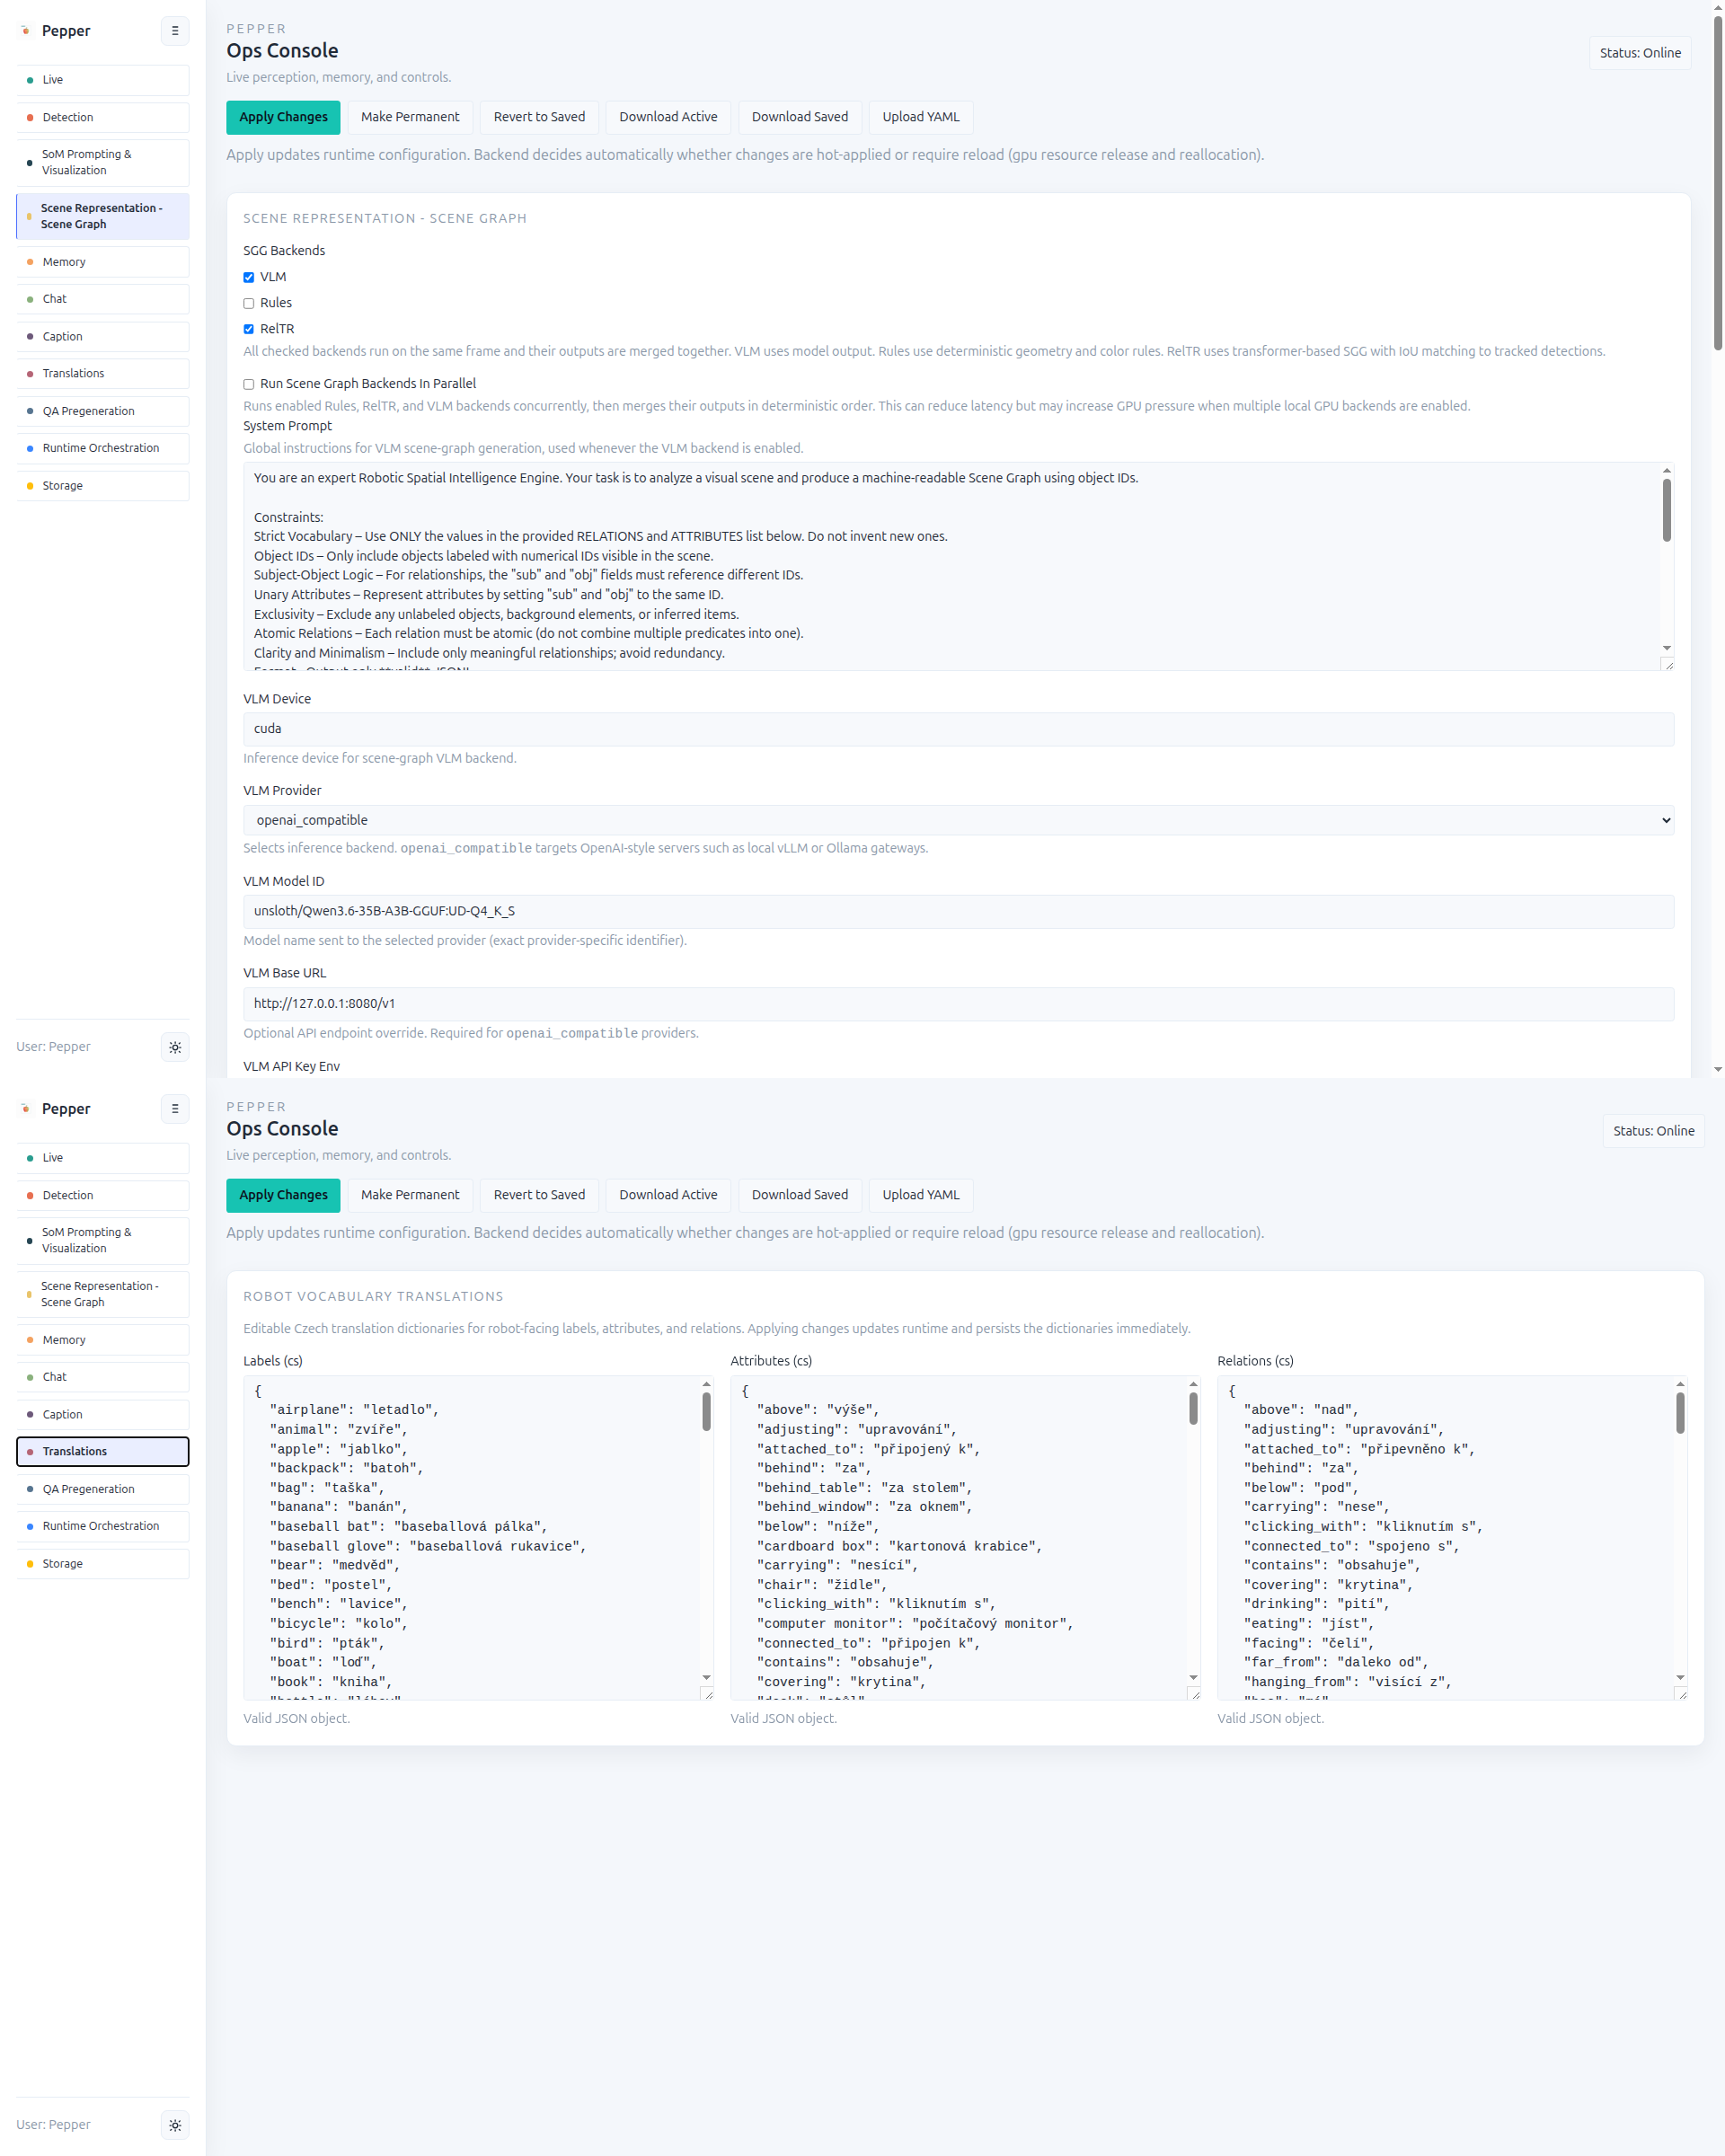
\includegraphics[width=1\linewidth]{pics/example_dashboard_translation_sgg_settings_vertical.png}
\caption{Dashboard configuration views for translation and scene graph generation. The server exposes runtime settings for label, predicate, and attribute translation, as well as scene graph backend and Set-of-Mark controls.}\label{fig:dashboard-translation-sgg-settings}
\end{figure}

Figure~\ref{fig:dashboard-translation-sgg-settings} shows two configuration views.
The translation settings allow labels, predicates, and attributes to be mapped for robot-facing language output.
Scene memory uses normalized internal names, while Pepper may need to speak or display a localized form.
Automatic translation is implemented with the \texttt{googletrans} library, which provides a Python interface to Google Translate functionality~\cite{googletrans_pypi_2026}.
The scene graph settings expose backend and prompting controls, including whether to use rule-based relations, RelTR, VLM scene graph generation, Set-of-Mark rendering, labels, boxes, masks, polygons, and related thresholds.

Configuration changes are divided into hot updates and hard reloads.
Thresholds, prompt paths, selected runtime flags, translation mappings, and some provider parameters can be pushed into a running runtime.
Changes that rebuild model objects require a hard reload.
In worker mode, a hard reload restarts the worker process so the public API remains separate from model teardown and GPU memory release.

The worker manager tracks worker state, process identifier, configuration version, inflight requests, health checks, idle shutdown, restart counts, crash counts, and last errors.
A robot system benefits from this separation because a local model process may become slow, fail, or retain GPU memory after a configuration change.
The public server can keep serving status and fallback responses while the worker lifecycle is managed separately.

The server implementation is therefore an integration layer under embodied constraints.
It does not contribute a new detector or a new language model.
Instead, it connects configurable perception, tracking, robot metadata fusion, scene graph generation, memory, and language services into a runtime that Pepper can call.
Chapter~\ref{chap:robot_side_rewrite} describes the other half of the system: the robot client that collects observations, manages turns, speaks responses, and presents server memory through speech and tablet interaction.
